\documentclass[12pt,a4paper]{article}
% \usepackage[subpreambles=true]{standalone}
\usepackage[a4paper]{geometry}
\usepackage[utf8]{inputenc}
\usepackage[T1]{fontenc}
\usepackage[light]{CormorantGaramond}
\usepackage{import}

\linespread{1.25}

\usepackage{amsmath, amssymb, amsfonts, amsthm, mathtools}
\newcommand{\R}{\mathbb{R}}
\newcommand{\Z}{\mathbb{Z}}
\newcommand{\argmin}{\arg\!\min} % AlfC
\DeclareMathOperator{\tr}{tr}
\newcommand{\irchi}[2]{\raisebox{\depth}{$#1\chi$}}
\newcommand{\rchi}{{\mathpalette\irchi\relax}}
\usepackage{algorithm}
\usepackage{algpseudocode}
\usepackage{float}

\usepackage{microtype} %improves the spacing between words and letters

\usepackage{lipsum}
\usepackage{threeparttable}
\usepackage{tabularx}
\usepackage{multirow}
\usepackage{booktabs}
\newcommand{\tabitem}{~~\llap{\textbullet}~~}
\usepackage{graphicx}
\graphicspath{ {./pics/} {./eps/}}
\usepackage{epsfig}
\usepackage{epstopdf}

%%%%%%%%%%%%%%%%%%%%%%%%%%%%%%%%%%%%%%%%%%%%%%%%%%
%% COLOR DEFINITIONS
%%%%%%%%%%%%%%%%%%%%%%%%%%%%%%%%%%%%%%%%%%%%%%%%%%
\usepackage[dvipsnames]{xcolor} % Enabling mixing colors and color's call by 'svgnames'
%%%%%%%%%%%%%%%%%%%%%%%%%%%%%%%%%%%%%%%%%%%%%%%%%%
\definecolor{MyColor1}{rgb}{0.2,0.4,0.6} %mix personal color
\definecolor{MyColor2}{HTML}{A30073}
\definecolor{MyColor3}{HTML}{A3008F}
\newcommand{\textb}{\color{Black} \usefont{OT1}{lmss}{m}{n}}
\newcommand{\blue}{\color{MyColor1} \usefont{OT1}{lmss}{m}{n}}
\newcommand{\blueb}{\color{MyColor1} \usefont{OT1}{lmss}{b}{n}}
\newcommand{\red}{\color{LightCoral} \usefont{OT1}{lmss}{m}{n}}
\newcommand{\green}{\color{Turquoise} \usefont{OT1}{lmss}{m}{n}}
%%%%%%%%%%%%%%%%%%%%%%%%%%%%%%%%%%%%%%%%%%%%%%%%%%

%%%%%%%%%%%%%%%%%%%%%%%%%%%%%%%%%%%%%%%%%%%%%%%%%%
%% FONTS AND COLORS
%%%%%%%%%%%%%%%%%%%%%%%%%%%%%%%%%%%%%%%%%%%%%%%%%%
%    SECTIONS
%%%%%%%%%%%%%%%%%%%%%%%%%%%%%%%%%%%%%%%%%%%%%%%%%%
\usepackage{titlesec}
\usepackage{sectsty}
%%%%%%%%%%%%%%%%%%%%%%%%
%set section/subsections HEADINGS font and color
\newcommand*{\myfont}{\fontfamily{cmr}\selectfont}
\chapterfont{\myfont \color{MyColor1}}
\sectionfont{\myfont \color{MyColor1}}
\subsectionfont{\myfont\color{MyColor1}}  % sets colour of sections

%set section enumerator to arabic number (see footnotes markings alternatives)
% \renewcommand\thechapter{\arabic{chapter}.} %define chapters numbering
% \renewcommand\thesection{\arabic{section}.} %define sections numbering
% \renewcommand\thesubsection{\thesection\arabic{subsection}} %subsec.num.

%%%%%%%%%%%%%%%%%%%%%%%%%%%%%%%%%%%%%%%%%%%%%%%%%%
%		CAPTIONS
%%%%%%%%%%%%%%%%%%%%%%%%%%%%%%%%%%%%%%%%%%%%%%%%%%
\usepackage{caption}
\usepackage{subcaption}
%%%%%%%%%%%%%%%%%%%%%%%%
\graphicspath{{./figures/}} %Setting the graphicspath
% \graphicspath{{./figures/G&D/}} %Setting the graphicspath
% \captionsetup[figure]{labelfont={color=Turquoise}}

%%%%%%%%%%%%%%%%%%%%%%%%%%%%%%%%%%%%%%%%%%%%%%%%%%
%		!!!EQUATION (ARRAY) --> USING ALIGN INSTEAD
%%%%%%%%%%%%%%%%%%%%%%%%%%%%%%%%%%%%%%%%%%%%%%%%%%
%using amsmath package to redefine eq. numeration (1.1, 1.2, ...)
%%%%%%%%%%%%%%%%%%%%%%%%
\renewcommand{\theequation}{\thesection\arabic{equation}}

%set box background to grey in align environment
\usepackage{etoolbox}% http://ctan.org/pkg/etoolbox
\makeatletter
\patchcmd{\@Aboxed}{\boxed{#1#2}}{\colorbox{black!15}{$#1#2$}}{}{}%
\patchcmd{\@boxed}{\boxed{#1#2}}{\colorbox{black!15}{$#1#2$}}{}{}%
\makeatother
%%%%%%%%%%%%%%%%%%%%%%%%%%%%%%%%%%%%%%%%%%%%%%%%%%

\makeatletter
\let\reftagform@=\tagform@
\def\tagform@#1{\maketag@@@{(\ignorespaces\textcolor{red}{#1}\unskip\@@italiccorr)}}
\renewcommand{\eqref}[1]{\textup{\reftagform@{\ref{#1}}}}
\makeatother
\usepackage{hyperref}
\hypersetup{colorlinks = true, linkcolor  = black}

%% LISTS CONFIGURATION %%
\usepackage{enumitem}
\setlist[enumerate,1]{start=1}
\renewcommand{\labelenumii}{\theenumii}
\renewcommand{\theenumii}{\theenumi.\arabic{enumii}.}
\newcommand{\cri}[1]{\textcolor{MyColor2}{\textbf{(Cri says: #1)}}}

%%%%%%%%%%%%%%%%%%%%%%%%%%%%%%%%%%%%%%%%%%%%%%%%%%
%% abbreviations:
%%%%%%%%%%%%%%%%%%%%%%%%%%%%%%%%%%%%%%%%%%%%%%%%%%
\usepackage[acronym]{glossaries}
\newacronym{pca}{PCA}{Principal Component Analysis}
\newacronym{svd}{SVD}{Singular Value Decomposition}
\newacronym{gsp}{GSP}{Graph Signal Processing}
\newacronym{omp}{OMP}{Orthogonal Matching Pursuit}

%%%%%%%%%%%%%%%%%%%%%%%%%%%%%%%%%%%%%%%%%%%%%%%%%%
%% PREPARE TITLE
%%%%%%%%%%%%%%%%%%%%%%%%%%%%%%%%%%%%%%%%%%%%%%%%%%
\title{\blue Homework Network Science course - Part1}
\author{Cristina Gava\\%
Matr 1153449}
\date{\today}
%%%%%%%%%%%%%%%%%%%%%%%%%%%%%%%%%%%%%%%%%%%%%%%%%%
%
% \usepackage{afterpage}
%
% \newcommand{\blankpage}{\null \thispagestyle{empty} \addtocounter{page}{-1} \newpage}

\begin{document}
\maketitle

In this first part of the Homework, I focused on some of the main parameters presented in the course so far, in particular with respect to pdf estimation, assortativity value, clustering measures and ML fitting.

\subsection*{The dataset}
The dataset selected was taken from \cite{repo}: the network is the transformation of the temporal graph (seen as a sequence of timestamped edges) into a static graph concerning reachability. In such way the new static network has edges representing metaphoric (phone calls or emails) or plain physical proxhimity between two entities. Hence this temporal reachbility graph represents a sequence of contacts obeying time and so the fact that a user could have transmitted a piece of generic information to another user.

\subsection*{First network metrics}
First of all, the main metrics of the network have been extracted and are summed up in \autoref{tab:metrics}. As we can see from the table, the netowrk has a high variance and so a high spread value. This information can also be observed in \autoref{fig:pdf}, where the degree pdf spreads significantly along the x-axis, resulting in a high variation in the degree values we can find inside the network. In the same way, also the skewness has a high value, resulting in an asymmetric degree distribution unbalanced towards the lower degrees (reult confirmed also by the low average degree).

\begin{table}
\centering
\begin{tabular}{c|c}
  \firsthline
  Metric & Value\\
  \hline
    Average degree & $29.59$\\
    Number of links & $1862$\\
    Number of nodes & $3594$\\
    Nodes degree variance & $764.83$\\
    Nodes degree skewness & $2651.44$\\
    Inhomogeneity ratio $k$ & $25.8477$\\
  \lasthline
\end{tabular}
\caption{Network metrics concerning nodes and links number and the degree moments.}
\label{tab:metrics}
\end{table}

\begin{figure}
\centering
  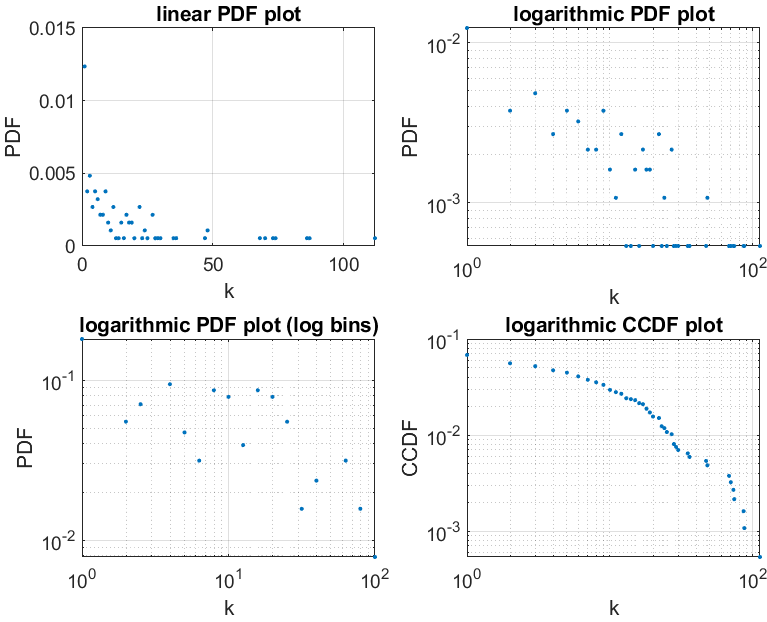
\includegraphics[width = 0.9\textwidth]{img/pdfPlots}
\caption{Plots of the various pdf functions: the normal one and the CCDF}
\label{fig:pdf}
\end{figure}

\subsection*{Power law exponent estimate}
For what concerns the power law exponent, \autoref{fig:ML} and \autoref{fig:MLest} show the $\gamma$ exponent estimation through ML fitting. The resulting value of $\gamma$ is $3.7736$ which does not go far from the classic hypothesis of $\gamma = 3.5$ and tells us that the network behaves as a common random scale-free network.

\begin{figure}
\centering
  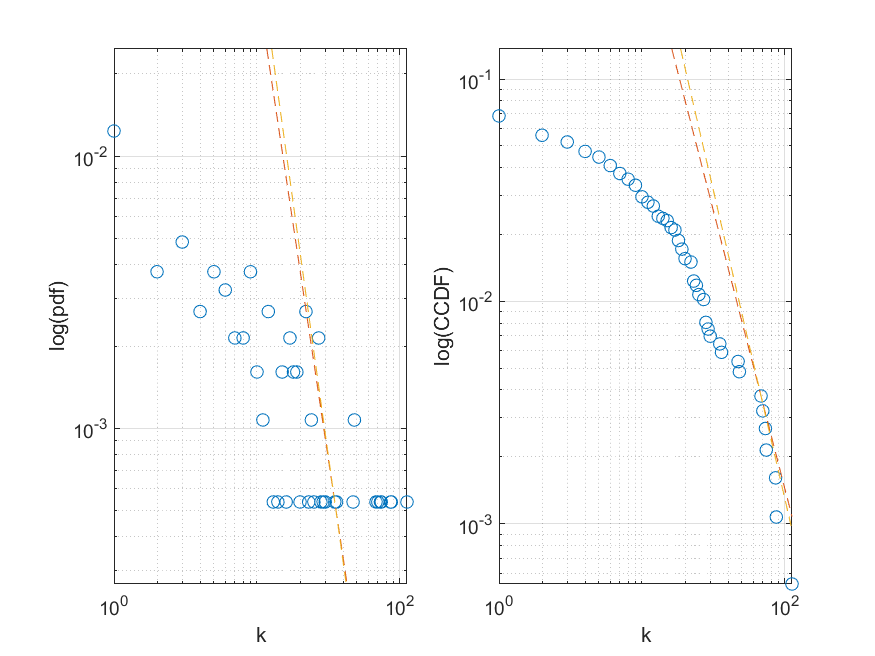
\includegraphics[width = 0.75\textwidth]{img/MLestimate}
\caption{Maximul likelyhood estimation}
\label{fig:MLest}
\end{figure}

\begin{figure}
\centering
\begin{minipage}[c]{0.47\textwidth}
  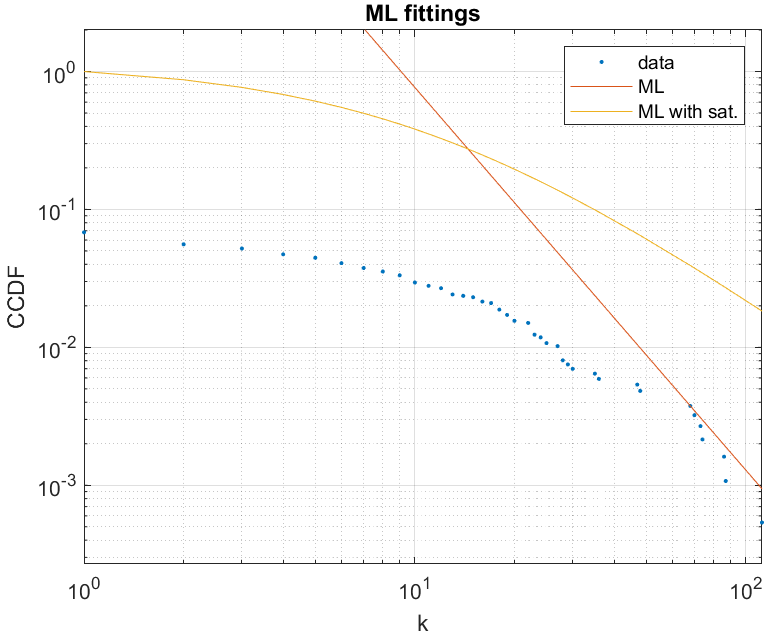
\includegraphics[width = 0.85\textwidth]{img/MLfitting}
\end{minipage}
\begin{minipage}[c]{0.47\textwidth}
  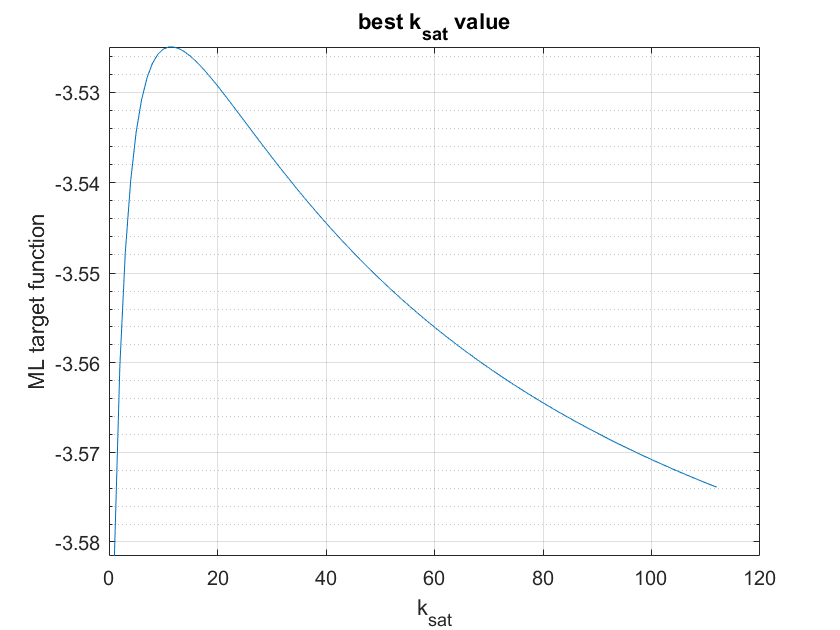
\includegraphics[width = \textwidth]{img/MLtargetFunction}
\end{minipage}
\caption{Maximum likelyhood fitting and target function estimation}
\label{fig:ML}
\end{figure}

\subsection*{Clustering coefficient}
Another interesting metric to look at is the clustering coefficient both for the general network and the connected-only component (\autoref{tab:clust}): the first value shows how the general network does not have a strong tendence to cluster, but looking at the biggest connected component we see that there is a high clustering behaviour. The behaviour is confirmed by \autoref{fig:netComm} and \autoref{fig:comm}.

\begin{table}[tb]
\centering
\begin{tabular}{c|c}
  \firsthline
  Average clustering coefficient & Average clustering coefficient\\
  of the full component &  of the major connected component\\
  \hline
$0.7160$ & $0.0253$\\
  \lasthline
\end{tabular}
\caption{Network clustering coefficients}
\label{tab:clust}
\end{table}

\begin{figure}
\centering
  \includegraphics[width = 0.75\textwidth]{img/ClusteringC}
\caption{Clustering coefficient pdf}
\label{fig:CC}
\end{figure}

\begin{figure}
\centering
\begin{minipage}[c]{0.47\textwidth}
  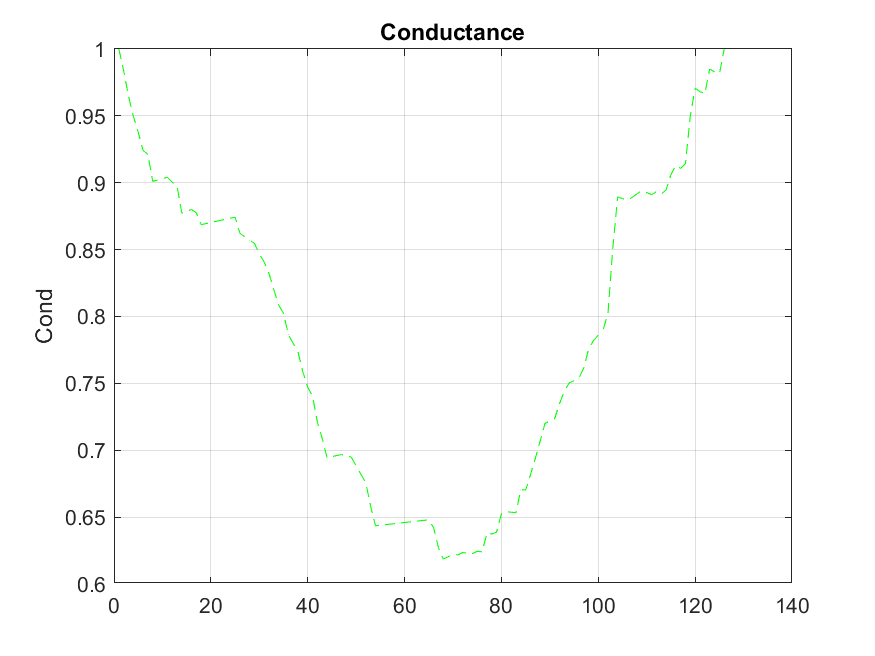
\includegraphics[width = \textwidth]{img/Conductance}
\end{minipage}
\begin{minipage}[c]{0.47\textwidth}
  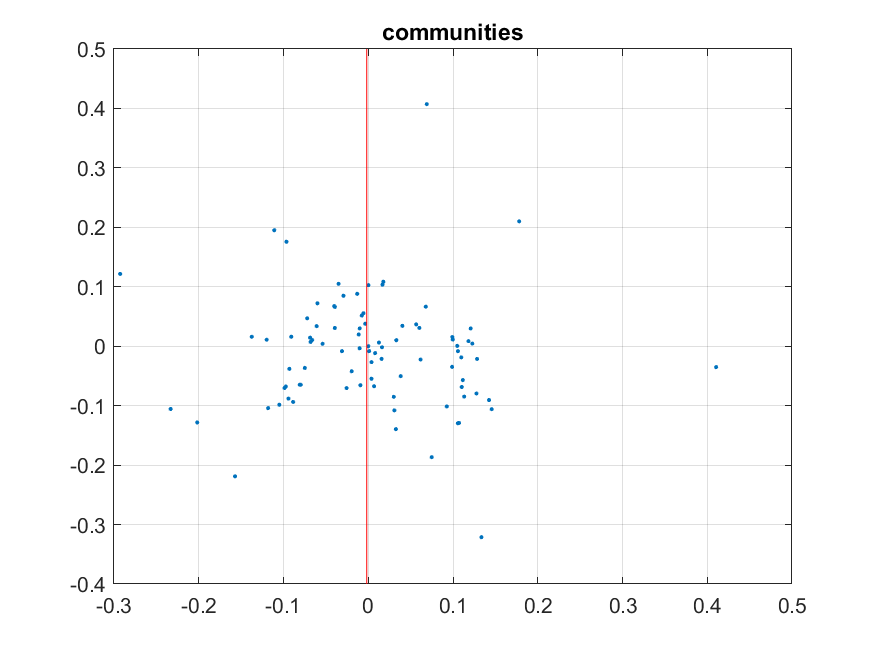
\includegraphics[width = \textwidth]{img/Communities}
\end{minipage}
\caption{Communities separation and representation}
\label{fig:comm}
\end{figure}

\begin{figure}
\centering
  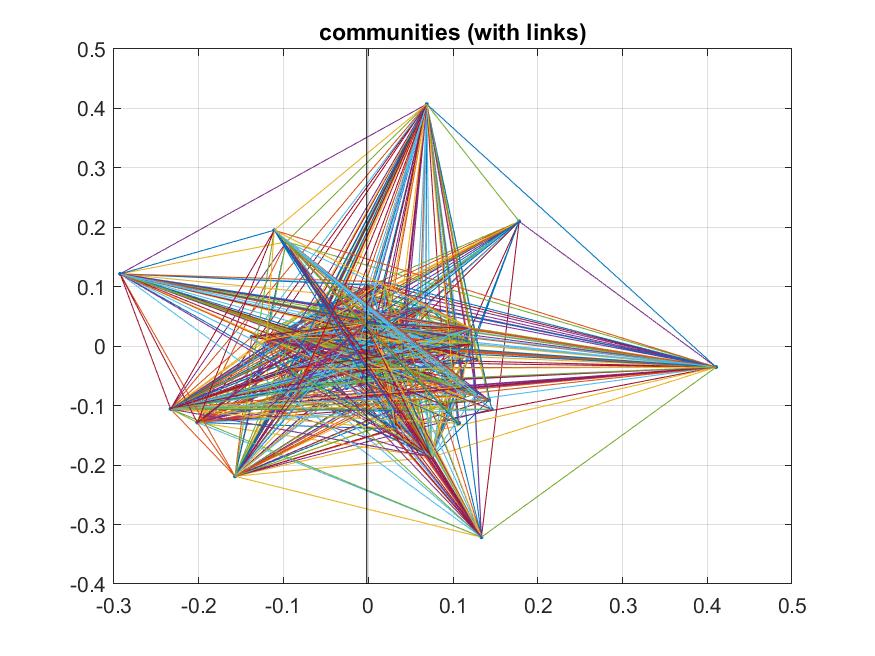
\includegraphics[width = 0.9\textwidth]{img/NetworkCommunities}
\caption{Network communities}
\label{fig:netComm}
\end{figure}

\subsection*{Assortativity values}
The resulting assortativity average values is $-0.46$, which means that the network has disassortative properties. The result is confirmed also by the neutral behaviour that emerged in the previous section and \autoref{fig:ND}. To be specific, the four graphs are equal, since the original network is undirected and the output degrees are specular to the input degrees. The effects of it, can be also observed in \autoref{fig:netComm} where we can foresee how nodes tend to connect to other elements having a different degree, resulting in a sort of "uniform mesh effect". In this case the structural cutoff comes around the degree magnitude $6$, which of course is smaller than the natural cutoff identifying the largest hub ($19.14$).

\begin{figure}
\centering
  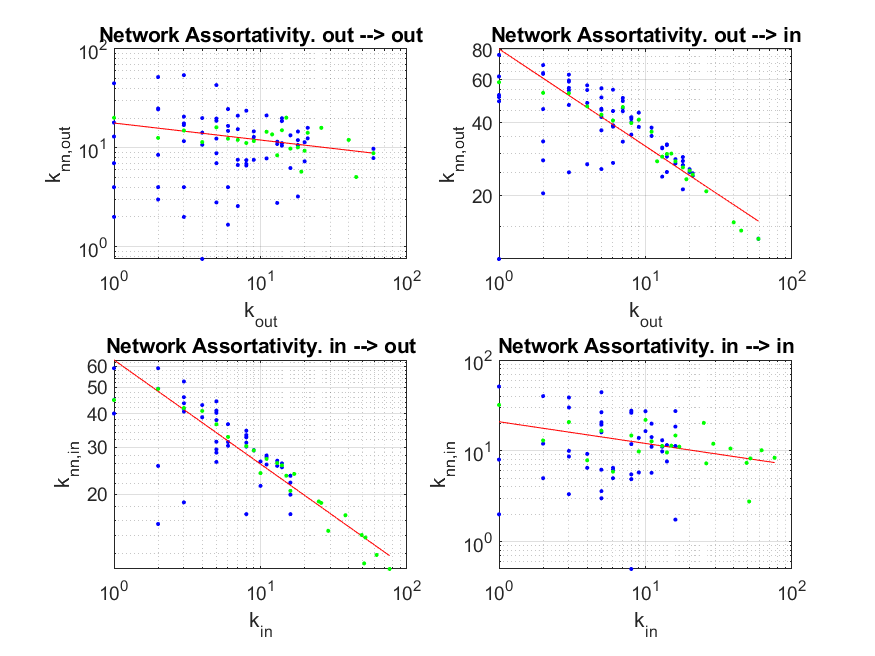
\includegraphics[width = 0.9\textwidth]{img/Assortativity}
\caption{Neighbouring degrees and assortativity. Assortativity interpolation = red line, average neighbouring degree = green dots, average degree of the neighbours = blue dots.}
\label{fig:ND}
\end{figure}

\subsection*{Network robustness}
Finally, attention must be paid to the network robustness, which can be summarized by the values of the inhomogeneity ratio and the breaking point estimate. The former is equal to $25.8477 > 2$ and so we confirm the presence of a giant component; the latter is equal to $0.2264$ which is rather low and signals a weak network. This conclusion is also confirmed by the low average degree of the nodes.

 \bibliographystyle{ieeetr}
 \bibliography{BibHack}
\end{document}
